\chapter{Binary Rewriting}
\label{binary_rewriting}

Binary rewriting is a software technique that transforms an executable by maintaining its original behaviour, while improving it in one or more aspects such runtime performance, security and reliability. The research literature is full of examples of binary-rewriting methods applied to a variety of topics, including optimization \cite{Romer97instrumentationand}, code instrumentation \cite{PEBIL, BIRD}, security enhancements \cite{vx32}, software caching \cite{Valgrind, DynamoRio} and emulation \cite{Qemu}. Consequent to the advantages of binary rewriting, numerous binary rewriters have been developed. Typically they fall into two main categories \emph{static rewriters} and \emph{dynamic rewriters}, which can be further subdivided according the approach taken in the rewriting process, \emph{full rewriting} where the entire file is rewritten and \emph{selective rewriting} where only relevant instructions are modified. 
\begin{description}

\item[Static binary rewriters] modify the executable file off-line allowing them to perform complex analysis and transformations. Due to their offline nature, \emph{relocation information} are required to identify code regions and address locations. The identification of the code region is necessary to ensure a fully disassembly of the binary file. Just merely disassembling  the entire code segment is an invalid solution, as  compilers often insert data within the code segment (such as jump table, padding bytes). The identification of address locations is required to adjust addresses during the relocation phase. The necessity of relocation information can be avoided using a selective binary-rewriting approach \cite{BIRD, seccompsandbox} as the original code remains the same to the greatest extend possible. Although this approach allows only minimal transformations such as, insertion of trampoline instruction to jump into an instrumentation block and peephole optimizations \footnote{A peephole optimization is an optimisation performed over a small set of instructions. It works by recognising sets of instructions that can be replaced by shorter or faster set of instructions.}.

\item[Dynamic binary rewriters] modify the executable during its execution. The key advantage of this methods is that it does not require any relocation or symbolic information as at runtime the identification of the code regions and the address locations is trivial. Unfortunately, dynamic rewriters introduce a remarkable overhead in the software execution as all rewriting operations occur at runtime. This makes infeasible to use a binary rewriter to perform complex transformation such as automatic parallelization as the overhead introduced is prohibitive. Consequent to this limitation, dynamic binary rewriters have been only employed for simply code instrumentation, and even in this case the overhead introduced is significant, for DinamoRIO 20 \% and PIN 54\%.
\end{description}

Although their limitations both static rewriting as well as dynamic rewriting can be successfully used to intercept system calls. The primary target of the system-call interceptor based on a binary rewriting approach described in this chapter, are ELF binary files that run on the Linux platforms, including both x32 and x64 architectures. Several instrumentation tools have been implemented \cite{PEBIL, BIRD, REINS}, but none of them has been exclusively designed for intercepting system call, though they can be used for accomplishing such task. 

A system call interceptor based on binary rewriting method, works by placing a branch instruction at each system call invocation within the application code which transfers control to the instrumentation code. As the previous interceptor mechanisms, a way to pre and post process a system call invocation is to be provided. This is accomplished by the instrumentation code, which executes a pre-routine, the system call and a post routine in sequence, and then return the control to the application. A routine must be designed in such way to ensure that the program state is preserved across its execution, for example saving the state registers in the stack before their execution and restoring their values after. This guarantees that the behaviour of the modified binary is the same as the behaviour of the original file.  In addition this system call interceptor must be able to identify all instructions that issue a request for a system call. Linux provides three different ways to invoke a system call:

\begin{description}

\item[Interrupts] have been used by Linux to implement system calls on all x86 platforms since its first release. To execute a system call, a user process can copy the desired system call number to the eax register ( both x32 and x64) and execute the instruction \lstinline$int 0x80$. This generates the interrupt 0x80 and the corresponding interrupt service routine is called. The task of this routine is to save the current state and call the appropriate system call handler based on the value of the eax register, further information regarding the implementation of this routine can be found in the \emph{entry.S} file in the source of the kernel. However, this mechanism has turned out to be really slow since Pentium IV architectures raising the need of a new efficient way to make system call. 

\item[Sysenter/Sysexit] instructions were introduced by Intel from the Pentium II and later CPUs to fix the overhead issue correlated to the use of interrupts as mechanism to invoke system call. \lstinline$SYSENTER$ can be executed by any application, while  \lstinline$SYSRET$ can only be executed by ring 0 programs.These instructions are used as a fast way to transfer control from a user mode (ring 3) to a privileged mode (ring 0), and back quickly, allowing a fast and safe way to execute system routines from user mode.These instruction directly rely on the \textit{Model Specific Registers} MSR which complicates that way to invoke a system call for an user, for a comprehensive explication of this mechanism refers to. Instead of using this mechanism directly, it is strongly recommended to use the system call entry/exit point exported in user space by the kernel since version 2.6. Kernel creates a single page in the memory and attaches it to all processes' address space when they are loaded into memory. This page contains the actual implementation of the system call entry/exit mechanism and it is called \emph{linux-gate.so}. This mechanism is usualy referred to as  \textit{Virtual Dynamically linked Shared Objects} (VDSO). It was first introduced to reduce the calling overhead on simple kernel routines ( i.e. \lstinline$getpid()$ and \lstinline$gettimeofday()$ ). Then it has been extend to work as a way to select the best system call method available in the architecture. This approach is available only on x32 architecture as x64 architecture  provides an afficient instruction that satisfy the system call invocation requirement.  

\item[Syscall] is a new instruction that has been introduced to support fast system call on x64 architectures. The number of the syscall has to be passed in register rax and its arguments go into the other general CPU registers, similarly to the interrupt approach. Returning from the syscall, register rax contains the result of the system-call. In addition, this new instruction fully supports six arguments, therefore no argument is passed directly on the stack.

\end{description} 

\begin{multicols}{3}

\begin{center}
\lstset{escapechar=@,style=asm}
\begin{lstlisting}[caption=\relax]
       movl    $len,%edx       
       movl    $msg,%ecx       
       movl    $1,%ebx        
       movl    $4,%eax         
       int 	   $0x80
\end{lstlisting}
\end{center}

\begin{center}
\lstset{escapechar=@,style=asm}
\begin{lstlisting}[caption=\relax]
     movl    $len,%edx       
     movl    $msg,%ecx       
     movl    $1,%ebx        
     movl    $4,%eax         
     call    *%gs:0x10
\end{lstlisting}
\end{center}

\begin{center}
\lstset{escapechar=@,style=asm}
\begin{lstlisting}[caption=\relax]
  mov    $1,   %rax          
  mov    $1,   %rdi         
  mov    $mes, %rsi     
  mov    $len, %rdx      
  syscall

\end{lstlisting}
\end{center}

\end{multicols}


A system call interceptor whose aim is to work with both x32 and x64 files must be able to correctly identify all previous instructions. When using a rewriting approach to intercept a system call, all libraries linked with this file must be instrumented as well to ensure that all system calls are caught. In the rest of this chapter we discus how to implement a system call interceptor using a binary rewriting approach, both dynamic and static. The section \ref{static_rewriting} introduces in more details techniques for static binary rewriting as well as issues that raise when a static rewriting is used for modifying ELF binaries within an architecture which supports  a set of instructions with different length ( such as Intel x86 and x86\_64 instructions). The section \ref{dynamic_rewriting} presents the general approach adopted by most of the dynamic binary rewriters. 

%%%%%%%%%%%%%%%%%%%%%%%%%%%%%%%%%%%%%%%%%%%%%%%%      STATIC REWRITTING %%%%%%%%%%%%%%%%%%%%%%%%%%%%%%%%%%%%%%%%%%%%%%%%%%%%%%%%%%%%%%
 
\section{Static binary rewriting}
\label{static_rewriting}

Static binary rewriting  is a powerful technique that transforms a binary file such as executables or libraries into a partially or totally new file. It allows to perform complex transformations (for example, automatic parallelization and porting binary between different architectures) as well as insert instrumentation code ( for example, for tracking purposes and security enhancements).Binary instrumentation offers a way for monitoring and controlling the execution of an instruction by allowing a extra code to be executed before or after of the instruction of interest. In this section, we describe how static binary instrumentation methods can be employed for the purpose of intercepting system calls. 
Although static code instrumentation introduces a minor number of changes than other  binary transformations, it must address all issues that affect a generic static binary rewriter. There are numerous challenges that a static binary rewriter must address in order to ensure effectiveness as well as correctness, the largest of which include how correctly interpret the instructions within the text segment, how to relocate the code maintaining the original behaviour,  how to accommodate the extra code needed by the extension routines and how to deal with variable-length instructions. 

%CODE DISCOVERY 
The first step of the rewriting process is the identification of all instructions, this process is usually referred to as \emph{code discovery}. Unfortunately, identifying all instructions cannot be accomplished merely by disassembling the text segment of a binary file, as compilers often produce a ELF binary whose text segment might contain data. Compilers usually store small data structures for providing convenient and efficient lookup of data such as identifiers and descriptors.In order to guarantee correctness of the executable, the portions of the text segment containing instructions must be identified as mishandling the data within the text segment might result in a different application's behaviour from the original one.

Diverse code discovery algorithms have been designed such as \emph{linear sweep},which disassemble each location in a linear fashion, but it does not guarantee 100\% disassembly. PEBIL uses a \emph{recursive traversal}, which identifies instructions by following only valid control flow edges. When control transfer instructions are encountered the algorithm continues discovery at the target location. A difficult problem is raised when an \emph{indirect} transfer instruction  ( e.g. \lstinline$jump _entry$ ) is identified as the target address is not identifiable statically. Different techniques have been developed to overcome this problem: 
\begin{itemize}
\item The easiest solution is to rely upon \emph{relocation entries}\footnote{Relocation entries are generate by the compiler when an absolute address is not available during compiling time, for example a function in a library}, unfortunately these are not included in commercial applications which narrows the applicability of this approach to few application. % I have the address of the library once the binary is full written

\item A different approach that does not rely on relocation entries is \emph{peephole examination},  used  in \cite{PEBIL}. Peephole examination consists of analysing the instructions nearby the indirect transfer function  in order to determine the target address of the indirect branch. This methods works, but it cannot guarantee a 100\% code discover. 
\end{itemize}  
    

Another problem to be addressed by a binary rewriter is that some instructions will contain operands which reference other location within the binary file. During the rewriting process the target of these instructions might change due to the relocation of the referenced block. Load and store instructions reference to locations containing data. Maintaining the original data segment and all data portions to their original address in the rewritten binary ensures that the these instructions can be relocated without changing their operand. While the operand of call and jump instructions contain the address of other instructions. If the address of the target instruction can identified statically, it can be adjusted to point to the relocated instruction. In the case this is not possible, the address of an indirect branch must be identified using the techniques discussed in the code discovery code phase. 

%RELOCATION 

A common approach to transfer control from the application code to the instrumentation routine is to replace a single instruction or more with an unconditional branch instruction that performs the transfer. On platform with fixed-instruction length instruction sets, such as MIPS, this approach is straightforward as all instructions can be replaced with another one without consequence. While on platform that uses a \emph{variable-length} instructions (i.e, x86), it may not always be possible to instrument an arbitrary point using a replacement technique. The amount of space available at the instrumentation point may be insufficient to accommodate an unconditional branch instruction, large enough to reach the instrumentation code. 

In x86 architecture both x32 and x64, an unconditional branch that uses an offset of 32 bits requires 5 bytes. The instructions of interest for a system call interceptor introduced in the previous chapter, are of size 1 for \lstinline$INT$ and 2 byte for \lstinline$syscall/systenter$.Therefore, simply replacing a system-call instruction with a branch to the instrumentation code is not feasible way to accomplish the instrumentation of all system call invocations  within the binary file. Different techniques have been used to transfer control to the instrumentation code. 

The first alternative is the method proposed by the BIRD project \cite{BIRD}. When the instruction at the instrumentation point is shorter than 5 bytes, additional bytes could come from the first one or two instructions immediately following or preceding the instruction at the instrumentation point as long as doing so does not affect the program’s execution semantics. In general, an instruction is safe to be replaced if it is not the target of any branch instruction. When BIRD cannot find any additional safe bytes to locate the branch instruction, it uses an interrupt instruction (i.e. \lstinline$int3$). This is instruction fits perfectly the instrumentation requirements because it is of a single byte size and transfers the control to an arbitrary routine via the exception handling facilities provided by the operating system. Unfortunately, it is unsuitable for accomplishing this efficiently as the INT introduces a large overhead due to the  heavyweight switch from user space  to kernel space  and back. A similar approach has been used in \emph{seccomsandbox} in a dynamic fashion.

Another option is the method presented in PEBIL\cite{PEBIL}, which is ideal for implementing a system call interceptor as it allows to insert a instrumentation code at an arbitrary points within the code application. The instrumentation code might be inserted before and after a system call instruction in order to control its execution. It uses a relocation and reorganization of the code at the function level in such a way that guarantee that 5 bytes are always available at the instrumentation point. This process consists of 4 different steps : 

\begin{enumerate}

\item \emph{Function Displacement} relocates the contents of a function to an area of the text section for use of the instrumentation test. Then the original entry point of the 									   function is linked to the new location via an unconditional branch.   
\item \emph{Branch conversion}	   The address of all branches are extended to use 32-bits offset in order to make them able to reach every target within the application memory 									   space ( typically 4Gb)  
\item \emph{Instruction Padding}   pads each instrumentation point with enough empty space so that a 5-byte instruction can be inserted.  
\item \emph{Instrumentation}	   replace the instructions at each instrumentation point with a branch that transfer control to the instrumetation code. 

\end{enumerate}

This method can be specialised for the purpose of system call interceptor by relocating only the function which contains a system call invocation. The padding instructions should be inserted before and after of a system call invocation. This allows a pre-routine to be inserted before the system call invocation and one just after the system call. Note in this case the instrumentation code does not execute the system call, while in the previous solution the system call instruction was rewritten and thus it must be executed by the instrumentation code. 


\begin{center}
\lstset{escapechar=@,style=asm}
\begin{lstlisting}[caption={Original instructions, x64 architecture}]
   	0000c000: <foo>: 
   	c000: 48 89 7d f8	mov %rdi, -0x8(%rdb)
   	c004: 5e			pop %rsi
   	c005: 75 f8			jne 0xc004
   	c007: c9			leaveq	
   	c008: c3			retq
   	
\end{lstlisting}
\end{center}

\begin{center}
\lstset{escapechar=@,style=asm}
\begin{lstlisting}[caption={Instructions after the rewriting process using a relocation code approach at functional level}]
00008000: <_rel_foo>: 
    8000: 90 90 90 90 90		[empty space]
   	8005: 48 89 7d f8				mov %rdi, -0x8(%rdb)
   	8009: 90 90 90 90 90 		[empty space]
   	800d: 5e								pop %rsi
   	800e: 0f 85 f8 ff ff ff	jne 0x8009
   	8014: 90 90 90 90 90 		[empty space]
   	8019: c9								leaveq	
   	801a: c3								retq

0000c000: <foo>: 
   	c000: 48 89 7d f8				jmpq 0x8000
   	c005: 90 90 90 90 			[empty space]
\end{lstlisting}
\end{center}


A totally different approach is that taken by binary rewriters that performs a full rewrite of the entire file as in the case of \emph{SecondWrite, REINS}.  In this case the problem of finding new space for the instrumentation code does not occur as it can be inserted during the rewriting process. Usually, following this approach a binary file is translated in a intermediary language, optimised and then translated back to the binary format. For example, \emph{SecondWriter} integrates binary rewriting technologies with the complier LLVM \cite{LLVM} by translating the binary file into LLVM's intermediate language IR. When the application is represented in IR, is passed through a series of analysis and transformation. The result then is given an code generation routine which recompile the application.   


%INSTRUMENTATION  
When a selective rewriting approach is used such as in PEBIL and BIRD, the problem to insert the instrumentation code within the binary file raises. In order to insert  additional code and data into an executable, additional space needs to be allocated within the executable in such a way that will be correctly treated at load time. Two additional segment should be inserted, one containing the instrumentation code and the other containing the data required by the instrumentation code. Furthermore, in the case of the PEBIL approach also the size of the code segment of the original binary should be modified as more space is needed to support the padding instructions. The ELF code segment might be extended using similar approach as for ELF injection \cite{ELF_inj}


The static binary approach for implementing a system call interceptor is more difficult to implement with respect to the previous approaches discussed in this document as require to  effectively solve all previous shortcomings as well as ensuring the correctness of the translated binary. In spite of the implementation difficulties, it provides a very low overhead due to the tracing mechanism, around 5\%. This intercepting mechanism does not require a monitor thread as the "monitoring code" resides in the same memory space of the controlled process. This is an remarkable advantage as it avoids all overhead due to accessing the memory of another process. 
Furthermore, it can be used also to implement a delegating architecture where a binary file is statically patched in order to issue requests for a system call to another process, as in the case of \cite{seccompsandbox,vx32} (they use a dynamic rewriting technique but the same approach can be implemented in a static manner). 

In the case of this typology of system call interceptor is used for security purpose,  it must be ensured that the instrumentation code cannot be rewritten by the application's instruction. This can be accomplished through \emph{software fault isolation} techniques \cite{sfi}. Only instrumenting the binary file is not sufficient to guarantee that all system calls are intercepted as, usually, programs use  wrapper functions provided by an external library to make requests for external resource. The libraries linked with the program must be instrumented as well. This can be done by implementing a specialised version of elf-loader, that inserts the code in the libraries before loading them in the memory. An alternative could be to statically link the program to the libraries and then perform the binary instrumentation on the entire file which contain application and libraries.        




\section{Dynamic binary rewriting}
\label{dynamic_rewriting}

Binary dynamic translation is a technique for dynamically modifying a program as it is being executed. It has been used in a variety of different areas: binary translation for executing programs on non-native CPUs  \cite{Ebcioglu97daisy:dynamic}; fast machine simulation \cite{Witchel96embra:fast}; and recently, dynamic optimization and safe execution \cite{DynamoRio, Strata, vx32}. In this section we describe how software dynamic translation can be used to implement system call interception.

Most software dynamic translators can be seen as a virtual machine. A dynamic translator fetches instructions, performs an application-specific translation, and then arranges for the translated instructions to be executed; these are roughly the same actions performed by a virtual machine. Implementing a system call interceptor application in a software dynamic translator is a simple matter of overriding the system call instructions (e.g. syscall) with a jump to a system call handling routine that performs user defined routine. This routine can be implemented in a similar fashion as those within a static binary approach, although when using a dynamic rewriting the problem of extending the ELF binary does not raise. A routine can be loaded in memory before running the application, and the memory segment on which it is located can be protected through the security features provided by the operating system (e.g. \lstinline$mprotect$). 

In a binary dynamic rewriter, the application’s code is translated on demand and thus the only translated code is the executed one, while in a static translator all the code must be already translated at run-time. This helps to handle easily indirect jumps as the operand of these instructions can be identified from the execution context. Dynamic binary rewriter is slower than one that use a static approach for two reasons.The first reason is that the translation is performed at run-time so the time spent translating the code is to be added to  the time spent executing it.This implies that the translation must be performed as fast as possible. It also means that the benefit from executing translated code must overcome, by far if possible, the time spent translating code. The second reason derives from the first, as the time spent in the translation must be the less possible most of operations available for a static rewriter cannot be performed following a dynamic approach as they would introduce a prohibitive overhead.  Although this limits the area of use of a dynamic rewriter, a system call interceptor based on dynamic rewriter can be implemented. 

A dynamic rewriter mediates the execution of an application by examining and translating its instructions. The basic unit of translation is a \emph{fragment}. A fragment is a sequence of instruction ending with a control instruction.  At the end of each basic block the application’s machine state must be saved and the control returned to the dynamic translator, this is referred to as \emph{context switch}. Translated instructions are held through the \textbf{translation cache} component. Basically it is contiguous region of memory reserved at the startup of the dynamic translator where all translated blocks are stored. This area of memory must be marked as executable as the translated code is executed in place once the translation is completed.  In order to have a good cache performance the translated block should be correctly aligned and allocated trying to enhance the locality of the code. When no more space is available in the cache for new fragments, the entire content of the cache is discarded. This is the cache management policy used by the Dynamo dynamic optimizer \cite{DynamoRio}. The advantages of this method are simplicity of implementation and fast fragment allocation and deallocation. The disadvantage is that when the executed portions of the application binary do not entirely fit within the cache, the simple eviction policy results in potentially useful fragments being discarded. 

The translating process starts capturing the application context, and searching for a translation for the block of source code which begins at the address pointed by the EIP register. If a translation for this instruction is found in the cache, a context switch restores the application context and starts executing the translated version.  If there is no translation in the cache, the space for a new fragment is allocated in the translation cache and the control is passed to the \textbf{translation unit}.

%FIGURE 
\begin{figure}[t]
\centering
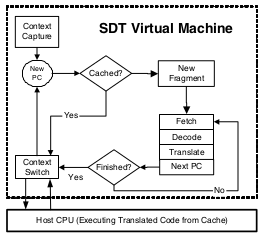
\includegraphics[scale=1]{Chapter3/Chapter3Figs/dynamic_algorithm.png} 
\caption{Dynamic translation algorithm}
\label{fig:dynamic translation algorithm}
\end{figure}

The task of the translation unit is to performs an application-specific translation and guarantee the correctness of the application. It starts fetching instructions from the address in the EIP register saved within the application context, until it reaches a  unconditional branch instruction or the maximum number of instruction per block.Than it decodes the instructions to be able to analyse them. It is particular interesting the approach taken by DynamoRio, which has developed an adaptive level-of-detail representation algorithm for decoding the instructions, where an instruction is only decoded and encoded as much as is needed. Note that there is not need to use a code discovery algorithm as in static approach because a fragment consists exclusively of instructions. Once the instructions are correctly translated,  they can be analysed for searching for instructions of interest. In the case of the system call interceptor the translation unit should search for instructions that might issue a system call request presented in \ref{binary_rewriting}. If one of those instructions is found, this must be overwritten with a jump to a system-call handling routine. Another advantage of performing binary rewriting at run time is that an instruction can always be substituted with another instruction even though the instruction set is of variable length. The translated instructions are copied in a new empty frame into the translation cache, therefore  there will always be enough space to allocate a jump instruction.   

During the translation process, the operand of a branch instruction must be adjusted to point to the translated block within the translation cache. This is ensue that only translated instruction are executed and therefore no system call invocation is missed. Usually the address are translated using a fast look-up hash table. 
If a translation for the target instruction does not exist, then the translation unit is invoked to translate the target block and insert it in the cache unit. Note that this approach might lead to duplicate code in the cache unit, for example when the operand of jump is an address pointing to an instruction in the middle of an block which has been already translated. A method used to improve the performance of handling branch instructions is to patch direct jumps and direct calls to avoid future lookups, this has been used in \cite{vx32, DynamoRio}. Unfortunately, patching cannot be used for indirect branches, including indirect calls and returns as their targets are variable. This hash table lookup for indirect branches, especially during return instructions, has been reported in \cite{vx32} to be the main source of slowdown in the execution of the dynamic rewritten binary. When the translation of a fragment is terminated, a context switch is performed and the application starts executing that fragment. The translation process is depicted in 


In the research literature, there are two examples of system call interceptor that are implemented following the approach previously discussed. The first is called Strata ,described in \cite{Strata}, where a system call interceptor has been used to ensure a safe virtual execution for an untrusted binary.  A 40\% of overhead is introduce in the execution of binary using the Strata tool, this is due principally to the rewriting process.  Strata has been implemented by following an easy approach concerning more about portability rather than performance and no optimizations have been introduced. A better and more complex example is implemented in vx32 \cite{vx32}. Vx32 is a lightweight sandbox that relies on segment protection as well as binary translation to confine an untrusted application.Vx32 is provided as static library that can be used to implement security tools. \emph{VxLinux} is a small system call interceptor implemented using vx32 library, it can be found at \cite{soft:vx32}. The interceptor mechanism is implemented following a delegating approach similar to that describe in chapter \ref{delegating_architecture}, it is able to run unmodified binary introducing an overhead spanning from 10\% to 50\% worst case. 




